
\documentclass[bachelor]{thesis-uestc}

\title{基于大语言模型增强的视觉语言导航研究}{TODO}
\author{李皓}{Li Hao}
\advisor{王鹏\chinesespace 教授}{Dr. Peng Wang}
\school{计算机科学与工程学院(网安学院)}{TODO}
\major{数据科学与大数据技术}{TODO}
\studentnumber{2020080903009}

\begin{document}
\makecover

\begin{chineseabstract}
视觉语言导航是具身智能的一个重要研究方向,在该任务中,智能体接收并理解指令,理解环境信息,并执行动作完成导航任务。在视觉语言导航任务中,大语言模型展现出强大的涌现能力,能够理解复杂场景和高级指令,借助内在知识做出导航决策。本文就大语言模型在视觉语言导航任务上的应用展开研究,提升视觉语言导航任务的性能。

本文首先就视觉语言导航的发展展开调研,分析了室内导航任务中的数据集,评价指标,以及基于预训练模型的传统方法。随后介绍了大语言模型在视觉语言导航任务中的三种适配模式:情景学习、思维链提示以及基于微调的方法,并研究了当前性能最好的传统模型增强方法。

为了提升大语言模型的提示效果,本研究在子指令生成和视点选择两个方向做了尝试。首先建立了一个子指令评估框架,并对比加入子指令前后传统模型的性能,随后利用标准子指令对LLM进行微调,提升了未见场景下的导航性能。

在视点选择部分,我们通过实验对比了微调前后的视点正确率,证明微调方法能够提升视点选择任务的性能。为了进一步提升视点选择的准确率,我们还提出逐层微调的方法,包括房间序列预测和视点选择两个阶段的微调。微调后模型在未见环境下能够完全预测正确$63\%$的房间类型序列,有效提升了LLM在视觉语言导航任务中的能力。

最后针对适配工作中存在的问题,我们提出了后续的改进方向,包括使用专用模型对视觉信息进行补充,以及构建思维链提示数据集进行微调等。

\chinesekeyword{视觉语言导航,大语言模型,计算机视觉}
\end{chineseabstract}

\begin{englishabstract}
Vision-and-Language Navigation (VLN) is a crucial research direction in embodied intelligence, where agents receive and understand instructions, comprehend environmental information, and execute actions to complete navigation tasks. In VLN tasks, large language models (LLMs) demonstrate a strong emergent capability, being able to understand complex scenes and advanced instructions and make navigation decisions leveraging intrinsic knowledge. This paper focuses on the application of large language models in VLN tasks to enhance task performance.

The paper begins with a survey on the development of VLN, analyzing datasets in indoor navigation tasks, evaluation metrics, and traditional methods based on pre-trained models. It then introduces three adaptation modes of LLMs in VLN tasks: In-context learning, chain of thought prompting, and fine-tuning-based methods, and explores enhancement methods that currently offer the best performance with traditional models.

To improve the prompting effect of LLMs, this study attempts two directions: sub-instruction generation and viewpoint selection. Firstly, a sub-instruction evaluation framework is established, and the performance of traditional models before and after the addition of sub-instructions is compared. Subsequently, LLMs are fine-tuned using ground truth, enhancing navigation performance in unseen environments.

In the viewpoint selection part, experiments comparing the accuracy rates before and after fine-tuning demonstrate that the fine-tuning method can improve the performance of viewpoint selection tasks. To further enhance the accuracy of viewpoint selection, we propose a multiple-layer fine-tuning method, including two stages: room sequence prediction and viewpoint selection. After fine-tuning, the model can correctly predict room type sequences in unseen environments with an accuracy of 63\%, significantly enhancing the capabilities of LLMs in VLN tasks.

Finally, addressing the issues in the adaptation work, we propose subsequent improvement directions, including the use of specialized models to supplement visual information and the construction of thought chain prompting datasets for fine-tuning.

\englishkeyword{Vision-and-Language Navigation, Large language models, Computer Vision}
\end{englishabstract}

\thesistableofcontents

\chapter{绪\hspace{6pt}论}

\section{研究工作的背景与意义}

视觉语言导航(Version-and-Language Navigation,VLN)作为具身智能(Embodied Agent)的前沿研究方向,涉及智能体与人类的交互通信,其中人类发布指令,智能体理解指令,观察环境,导航或与环境互动,最终完成任务。

VLN 任务将计算机视觉,自然语言处理等深度学习的研究方向结合在一起,提升了智能体对于视觉和语言信息的联合感知能力,能有效拓宽智能体的应用场景。在导航过程中,智能体处于特定环境中,收到指令,并通过某种形式探索环境,规划路线,最终完成导航任务。自然语言指令贴合人和智能体交互的一般场景,而视觉信息帮助智能体交互时理解周围环境。

在日常任务处理,或者是抢险救灾等情况下,能够自主进行导航任务的机器人将有助于解放人的劳动,保障人的生命安全。


\section{视觉语言导航的国内外研究历史与现状}
随着人工智能技术的发展,研究者们开始逐渐探索人工智能理解物理世界,并与之互动的能力,这一研究领域就是具身智能。这一方法旨在将人工智能系统和真实或模拟环境集成,使其能够执行同人类相似的任务。为了实现这一目标,具身智能需要具有类似人的认知能力,以及在现实世界中的交互能力。目前,具身智能已经成为下一代人工智能理论和应用突破的关键前沿。

视觉语言导航(Vision-language navigation)任务是具身智能的一个重要研究防线,融合了人工智能,自然语言处理,计算机视觉,机器人技术等领域。其目标是利用智能体理解自然语言指令和解释视觉信息,使得智能体能够在虚拟或者是真实环境下进行导航,执行指令任务。

视觉语言导航任务由 Anderson 等人\cite{anderson2018visionandlanguage} 首先提出,利用 MatterPort3D 环境构建出了 R2R 数据集。Matterport3D 数据集在90个不同风格的建筑下采样了10800个RGB和深度图像,提供了丰富的真实场景信息。R2R 数据集由文本指令和对应的视点轨迹构成,平均每条指令包含29个单词,视点和Matterport3D\cite{changMatterport3DLearningRGBD2017}中的采样点相对应。此外,为了模拟智能体同环境交互的行为,该工作还构建了相应的执行模拟器 MatterPort3D Simulator。

此后在该数据集的基础上,更多相关的室内导航数据集被提出。在 R2R 的基础上衍生出若干变体,如Room-across-Room \cite{ku2020roomacrossroom},Landmark-R2R \cite{heLandmarkRxRSolvingVisionandLanguage2021}等,在指令轨迹、多文化环境和地标信息的角度扩展了原始数据集。一些数据集将眼光从室内移向室外,如 TOUCHDOWN 数据集\cite{chenTOUCHDOWNNaturalLanguage2019}利用纽约市的街景信息,将室内环境扩展到室外。ALFRED\cite{shridharALFREDBenchmarkInterpreting2020}和REVERIE\cite{qiREVERIERemoteEmbodied2020}数据集引入了和物体之间的交互任务,不仅仅要求智能体导航到目标所在的地点,还需要和指定的额物体进行交互(拾取、互动等),有效扩展了智能体的行动空间,更加贴近应用场景。

解决视觉语言导航任务的关键在于解决三个主要问题。首先是多模态的融合与理解,智能体需要使用视觉和语言信息,对复杂指令和动态场景进行有效集成。其次,智能体的算法需要具有强大的泛化能力,并优化计算的效率,面对多样的场景和任务需要保持有效,同时尽可能降低计算的需求。最后,由于模拟环境和有限的数据集,智能体在实际应用上存在困难。

目前基于学习的视觉语言导航任务集中于三种解决思路,包括基于表示学习,基于决策和策略学习以及数据驱动的方法三个部分。随着大语言模型的发展,LLM用于增强导航模型的也成为一个重要的研究方向。为了深入理解这些方法如何共同推动视觉语言导航技术的发展,接下来将逐一介绍这些方法。

\subsection{基于表示学习的方法}
   基于表示学习的核心任务是加深智能体对于各个模态之间关系的理解,尤其是指令的词汇与环境感知特征之间的相互动作。有效的表征学习能够帮助智能体在处理图像,指令和导航动作时建立视觉语言描述和视觉信息的联系,增加复杂场景下的导航能力和决策效率。

   表示学习的方法由单模态到多模态的演化过程。在视觉提取方面,特征提取方法由 ResNet\cite{he2015deep} 演变到 Vision Transformer\cite{dosovitskiyImageWorth16x162021} 等模型;指令理解方面,基于 RNN\cite{Sherstinsky_2020} 的方法逐渐被基于 BERT\cite{devlinBERTPretrainingDeep2019} 的方法取代。这些进展为基于学习的方法奠定了基础。

   多模态的联合表示方法成为目前解决视觉语言导航任务的一个主流方法,视觉语言预训练模型提供了二者的高效表示。一种常见的方法是利用 ViLBERT 等视觉语言预训练模型来初始化智能体,并进行下游任务训练来适配到视觉语言导航任务中。

   多模态联合表示的一个重要方法是引入图这一数据结构来融合指令和导航观察,利用节点间关系来提供清晰的语义表示。图记录了导航过程中的位置信息,帮助预测动作,记录先前的导航位置,提供回溯选择。

   在面对精简的高级指令时,导航任务的难度提高,尤其是在智能体面对未曾探索过的场景或者是指令时,往往不能够精确的到达目标地点。基于导航图的方法如HAMT\cite{chen2021history},DUET\cite{chenThinkGlobalAct2022} 等方法,利用BERT\cite{devlinBERTPretrainingDeep2019} 等预训练模型将指令映射为嵌入向量,同导航时的视觉特征一起协同训练,构建出导航策略。这些方法提供了全景视图,历史全景等信息进行分层编码,构建了完整的导航历史来进行决策。

\subsection{基于决策和策略学习}
   视觉语言导航任务面对多样化的行动选择和复杂的环境状态,策略学习提供了一系列方法帮助智能体确定最佳的导航选择。策略学习包含三种:基于路径规划的方法、基于强化学习的方法和基于先验探索的方法。

   基于路径规划的方法常常在给与详细指令的情况下运用。语言指令提供了智能体在执行过程中能够看见的关键物体,以及需要遵循的路线描述。智能体需要严格遵循指令的轨迹移动,才能到达目标位置。为了使智能体保持在规定的轨迹上,需要对轨迹进行分段规划,提供合适的停止信号,能有效提升智能体导航的效率和准确性。

   由于VLN本质上作为一个序列决策问题,其结构天然适合被构建为一个马尔可夫决策过程(MDP)。因此,为了更加有效的学习VLN任务,强化学习被应用在该领域。然而,强化学习方法面对的一大挑战在于奖励信号的稀缺,VLN智能体只有当一次导航结束之后才能够获知成功或者失败。也就是说,对于每一次行动,并没有明确的奖励信号作为反馈。因此设计奖励机制是强化学习方法的关键所在。

   视觉语言导航任务的模型在熟悉的场景中具有较好的效果,但是这种能力难以推广到未知场景。预先探索的方法首先探索未知环境,从而缩小未见场景和见过场景中的性能差距。在预先探索过程中,智能体利用记忆的方式适应周围环境,构建了未见环境的地图,从而能够有效提升导航性能。

\subsection{数据驱动的方法}
   基于数据驱动的方法利用现成的数据合成为视觉语言导航任务数据。有效扩展了导航数据集,还增强了模型在新环境中的泛化能力。例如,R2R 数据集仅仅包含21567条数据,稀缺的数据增加了模型性能的提升,因此需要在此基础上对指令进行合成与扩展。

   基于多任务和迁移学习的方法也能够有效缓解室内导航数据少的问题,从其它任务上学习到的知识有益于视觉语言导航任务的完成。此外,利用课程学习的方法对导航任务按照难度递增的顺序进行排列,也可以有效的适配复杂的室内导航任务。

\subsection{基于大语言模型增强的方法}

GPT3\cite{ouyangTrainingLanguageModels2022} 等大语言模型(LLM)的发展,为视觉语言导航的研究带来了新的方向,基于少样本甚至无样本的室内导航成为可能。周围的环境信息输入LLM 中,并且利用LLM做出导航决策,即使是面对未见的场景,也可以通过提示工程来引导生成导航轨迹。NavGPT\cite{zhouNavGPTExplicitReasoning2023a} 利用大语言模型(GPT-4\cite{openaiGPT4TechnicalReport2024})进行导航规划,分解导航目标,理解导航进度,完成导航任务。受限于其总结导航历史的方式,该模型在R2R数据集中的细粒度导航指令表现较好。另一个较为突出的工作是 MapGPT\cite{chenMapGPTMapGuidedPrompting2024},利用图结构维护导航点的联通关系,通过简单修改提示词即可在R2R 和 REVERIE 数据集上切换,并且取得了比 NavGPT 更好的效果。基于LLM的模型展现出极大的应用前景,但基于这些方法的性能仍然不能超越基于学习的方法。

  
基于上述分析,一种可行的探索方向是将 LLM 同基于训练的模型相结合,从而在导航的关键指标上达到更好效果。MiC\cite{qiaoMarchChatInteractive2023} 将 GPT-2\cite{brownLanguageModelsAre2020} 同 HM3D-DUET \cite{chenLearningUnlabeled3D2022} 相结合,在感知到房间类型发生变化时根据环境观察动态生成子指令,同高级指令一同完成导航任务。该方法在平均带权路径指标下取得了最好效果。想要改进LLM生成的子指令质量,如何评估LLM在子指令生成方面的效果成为一个有挑战的问题。为此,本研究希望探索一种基于导航策略融合的方法,对LLM在VLN任务下的性能进行调优,并探索一种高效的融合方式。
\section{本文的主要贡献与创新}

本文的主要贡献和创新如下:
\begin{enumerate}
    \item 搭建了视觉语言导航子指令评估框架,将LLM同传统模型结合起来,构建数据集对子指令生成任务进行微调,提升了传统模型的效果。
    \item 探究LLM直接生成视点选择的方法,对比微调前后准确率的变化。
    \item 提出一种分层微调的方法,有效提升了LLM预测房间类型序列的能力。
\end{enumerate}
\section{本论文的结构安排}

本文的章节结构安排如下:

第一章首先介绍了视觉语言导航任务的背景和意义,并阐述了该领域近年来的发展现状。

第二章介绍了视觉语言导航任务主要的几个数据集,以及导航的性能评价指标。最后介绍了基于学习的导航方法。

第三章介绍了大语言模型在视觉语言导航任务的适配方法,并介绍了该领域下前人做的工作。

第四章从子指令生成和视点选择两个角度,进行LLM在视觉语言导航任务的适配实验,并展现了实验效果。

第五章总结了本文的主要工作,提出了未来可能的改进方向。

\chapter{视觉语言导航框架与基础模型}

在本章节,我们将首先介绍视觉语言导航任务的框架,随后将详细探讨视觉语言导航的基础模型。框架部分将首先介绍视觉语言导航任务的定义,随后介绍视觉语言导航数据集R2R,REVERIE,以及FG-R2R,包括其特点和差异,最后将介绍视觉语言导航任务的衡量标准。在基础模型部分,我们将将介绍近年来在 REVERIE 数据集上取得较好性能的方法。

\section{视觉语言导航任务定义}

视觉语言导航任务的目标是构建一种智能体,能够使用自然语言和人类沟通,并且在真实的环境中导航的具身智能体。该任务涉及预言者(通常是人类)、智能体和环境的任务。智能体和预言者使用自然语言进行交互,智能体可能请求指导,预言者做出响应,智能体根据接受的指令和周围的环境观察来进行导航,并和环境进行互动完成导航任务。预言者观察环境和智能体的状态,在必要时刻和环境互动以帮助智能体。预言者,智能体和环境三者的关系如图\ref{orace}\cite{guVisionandLanguageNavigationSurvey2022}所示。

在本研究中,视觉语言导航(Visual Language Navigation, VLN)任务被定义为智能体在离散环境中接受导航指令,观察环境状况,并完成导航任务。

智能体所处的离散环境可以被建模为一个无向图 \( G = \{V, E\} \),其中 \( V = \{V_i\}_{i=1}^{K} \) 表示 \( K \) 个可导航节点,\( E \) 表示连接这些节点的边。边代表相邻两个节点的可达性。在导航任务开始时,智能体并没有完整的环境地图,需要在探索过程中记录房间布局信息。

智能体(agent)配备了一个RGB摄像头和一个GPS传感器,并在一个之前未见过的环境中的起始节点初始化。智能体的目标是解释自然语言指令,并沿着图 \( G \) 导航到目标位置,找到指令中指定的对象。

自然语言指令由 \( L \) 个单词组成,其词嵌入表示为 \( W = \{w_i\}_{i=1}^{L} \)。在每个时间步 \( t \),智能体接收到当前节点 \( V_t \) 的全景视图和位置坐标。全景图被分割成 \( n \) 个图像 \( R_t = \{r_i\}_{i=1}^{n} \),每个图像由一个图像特征向量 \( r_i \) 和一个唯一的方向表示。为了实现细粒度的视觉感知,使用标注的对象边界框或自动对象检测器从全景图中提取了 \( m \) 个对象特征 \( O_t = \{o_i\}_{i=1}^{m} \)。

智能体还知道其邻近节点 \( N(V_t) \) 的一些可导航视图以及它们的坐标。\( N(V_t) \) 的可导航视图是 \( R_t \) 的一个子集。在步骤 \( t \) 时,智能体的可能本地动作空间 \( A_t \) 包括导航到 \( N(V_t) \) 中的 \( V_i \) 或在 \( V_t \) 处停止。一旦智能体决定在某个位置停止,它需要预测全景图中目标对象的位置。
\begin {figure}[h]
\centering % 居中显示
\includegraphics[width=0.7\textwidth]{5253-050520.png}
\caption{视觉语言导航任务中的实体互动图} % 标题
\label{orace}
\end {figure}
\section{数据集}

本研究主要就R2R,REVERIE以及FG-R2R数据集进行研究。R2R 为视觉语言导航任务提供了详细的指令,REVERIE 数据集和 R2R 共享相同的轨迹和环境,但指令更为精简,需要智能体探索环境。FG-R2R 数据集提供了R2R 指令细粒度的切分,并标记了对应的子指令序列。本研究将利用这三个数据集,探索智能体在REVERIE高级指令下,面对未见场景的导航性能。

\subsection{R2R 数据集}
R2R数据集是首个提出视觉语言导航任务的数据集,数据由详细的指令和指令对应的路径构成。指令由人工标注,详细描述了从起点到终点经过的移动过程,包含地标信息,房间功能,以及关键物体的特征描述。每条指令平均长度为29个词。路径在Matterport3D采集的室内场景构建而来,每条轨迹由离散的导航点构成。在每个离散的导航点处,智能体都能获得当前的全景观察,包含RGB色彩信息以及深度信息,如图\ref{r2r}所示。

\begin {figure}[h]
\centering % 居中显示
\includegraphics[width=0.8\textwidth]{4556-042815.png}
\caption{视觉语言导航任务样例} % 标题
\label{r2r}
\end {figure}

视觉语言导航任务最终希望让智能体在现实场景中导航,完成任务,但受限于成本限制,使用模拟环境进行室内环境导航更可行。R2R 数据集基于 Matterport3D 数据集构建了 Matterport3D simulator ,用于模拟智能体在室内导航场景下的移动。智能体在环境中的姿势由三个维度决定:视点$V$,航向角(heading)和俯仰角决定,在每个姿势下都能获得第一人称RGB-D图像和周围可导航的视点。智能体在环境中只能在相邻视点之间进行移动。

R2R数据集在90个不同的室内场景构成,场景可能存在多层,大部分是私宅,同时包含办公室,教堂等场景。一个场景平均有117个视点,可能覆盖多个楼层或是多个相同类型的房间,如图所示。数据集划分为四个部分,训练集(training set),已见-验证集(valid seen set),未见-验证集(valid unseen set),测试集(test set)。其中已见/未见数据集的区别在于,已见数据集在训练集中的相同场景下构建了新的指令,训练过程中智能体已经见过所处的环境,而未见测试集模拟环境陌生指令陌生的情况,更加贴合测试环境。

% \textcolor{red}{室内场景提示样例}

R2R 数据集在导航开始时提供了详细的指导,描述导航动作,智能体需要根据周围环境观察判断当前的导航指令的执行情况,并在合适的时机做出动作,直到指令执行完成后停留在终点。考虑人和智能体交互的过程,人们在提出任务时,往往不会用如此详细的方式给出指令。而 REVERIE 数据集的提出,弥补了高级指令的缺失。

\subsection{REVERIE 数据集}
REVERIE数据集提供了更加简洁直接的高级指令,但在任务上有所不同,R2R要求导航到场景中的某个地点,而REVERIE要求导航到某个不可见的物体处,这需要智能体利用周围环境知识推断物体可能所处的可能位置,并且根据语言指令来准确识别物体。相较于 R2R 数据集而言,REVERIE 数据集的单词数量更少,精简了具体的指引,强调最终的目标位置。因此REVERIE中的指令被认为是高级指令,R2R为细粒度指令。对于同一轨迹下的高级指令和细粒度指令之间的区别,如表\ref{rvr2r}所示。

\begin{table}[h]
    \centering
    \caption{REVERIE 和 R2R 指令对比}
    \label{rvr2r}
    \begin{tabular}{@{}p{0.45\linewidth}p{0.45\linewidth}@{}}
    \toprule
    \textbf{REVERIE} & \textbf{R2R} \\ \midrule
    Go to the first floor stairs that have the triangle designs on them and hang onto the rail as you go up the stairs & You're in a bathroom, turn to the right and walk through the doorway. Walk over the carpet and to the colorful stairs. Walk up a step and then wait. \\
    Go to the living room on level 1 and remove the nearest pillow from the couch that is closest to the dining room & Go down the hallway and turn left when you get to a door. Pass one pot with a plant and before you get to the second one turn left on the second entrance. Pass the table and chairs and turn right. Head into the living room and wait by the fireplace. \\
    Go to the 2nd floor bathroom with the gold and white striped shower curtain and polish the mirror over the sink & Turn to the right and walk out of the bedroom door. Turn left once you get into the hallway. Then turn right at the first door. You'll be looking into the bathroom. Stop when you get into the doorway. \\
    \bottomrule
    \end{tabular}
    \end{table}

REVERIE 数据集以远程物体作为指令主体,需要智能体理解指令的最终意图,也就是说,需要智能体自主决策导航路径。面对这样的场景下,智能体需要具有规划,记忆,以及回溯的功能。智能体接受指令后需要对全局的导航动作进行规划,而这正是REVERIE数据集没有提供的。在执行每一步之后,智能体都需要记录维护走过的动作,观察到的场景信息,并在下一步动作之前分析状态,做出继续前进或者是回溯的选择。本人将在后续章节对此展开详细叙述。

\subsection{FG-R2R 数据集}
为了更好的研究 R2R 指令的构成,以及指令序列和视觉序列之间的对应关系,Hong 等人\cite{hongSubInstructionAwareVisionandLanguage2020}提出了 Fine-Grained R2R 数据集(FG-R2R),为R2R数据集提供了细粒度的注释。具体来说,FG-R2R 数据集将原始 R2R 数据集中的指令进行启发式切分,将一条原始指令切分为若干条较短的子指令。这些子指令要么指向某些关键物体或者地标,要么描述关键动作。在获取子指令后,FG-R2R 对环境中的视点做了标注,利用模块化注意力机制匹配子指令片段和对应的导航轨迹片段。FG-R2R 数据集将在子指令微调部分发挥作用,作为学习样例引导LLM从高级指令生成对应的子指令。

\section{视觉语言导航性能指标}

在视觉语言导航任务中,对智能体的评估非常重要。为此,数据集提供了一系列指标,从多角度衡量智能体准确理解指令和在复杂场景下的导航能力。本节将详细介绍这些评估指标,并讨论如何利用这些指标分析智能体的性能。

\begin{itemize}
    \item 成功率(Success Rate,SR)
    
    成功率衡量任务最后成功的比例,智能体移动到目标位置3m以内停止,就视为成功。成功率由式计算。
    \begin{equation}
        \text{SR} = \frac{\text{成功次数}}{\text{总任务次数}}
    \label{sr}
    \end{equation}
    \item 预知成功率 (Oracle Success Rate, OSR)
    
    智能体有时导航到了目标点,却没有停止,而是继续行动,走到了错误的地方。在有外界指导的情况下,智能体可以在成功地点停止。为了衡量这种情况,研究者设置了预知成功率这一指标,统计整个轨迹上预知成功的次数。智能体在一次尝试的轨迹中,有任意视点能观察到三米以内的目标物体,则视为预知成功。预知成功率由式计算。

    \begin{equation}
        \text{OSR} = \frac{\text{预知成功次数}}{\text{总任务次数}}
    \label{OSR}
    \end{equation}


    \item 轨迹长度(Trajectory Length, TL)
    
    智能体在所有尝试过程中的平均轨迹长度,由式计算,
    \begin{equation}
        \text{TL} = \frac{\sum_{i=1}^N l_i}{N}
    \label{tl}
    \end{equation}

    其中 $l_i$ 代表第$i$ 次尝试下从开始到智能体停止的轨迹长度,$N$ 代表总尝试次数。

    \item 路径长度加权成功率 (Success weighted by Path Length, SPL)
    
    SPL 作为一个综合指标,考虑了成功率(SR)以及轨迹长度(TL)。考虑这样的场景,如果仅仅使用成功率衡量智能体的性能,一个显而易见的方法是采用图遍历算法,将室内场景遍历一遍,再选择置信度最高的点作为停止点。这样虽然能带来成功率的数值提升,但是却违背了探索(Exploration)和利用(Exploitation)的平衡关系。我们希望智能体执行指令时,兼具效率和准确性。式为SPL的计算方法:

    \begin{equation}
        \text{SPL} = \frac{1}{N} \sum_{i=1}^{N} S_i \frac{l_i}{\max(p_i, l_i)}
    \label{spl}
    \end{equation}

    其中,\( N \) 是尝试次数,\( S_i \) 是第 \( i \) 次尝试的成功标志(成功为1,失败为0),\( l_i \) 是完成指令的最短路径长度,\( p_i \) 是智能体实际走过的路径长度。
\end{itemize}

上述四个指标反映了导航的性能,成功率相关指标越高越好,轨迹长度则是越短越好。路径长度加权成功率平衡了成功率和路径长度的关系,反映了探索和利用的平衡。后续的工作围绕这些指标,探索不同的模型架构和训练方法,提出了视觉语言导航的新解决思路。

\section{基于学习的方法}

解决视觉语言导航任务需要解决两个关键问题,轨迹记忆和导航规划。智能体在导航过程中需要通过记录走过的路径,维护视点的连通性,先前的工作往往是以RNN,LSTM等网络作为记忆, 这些方法往往将过去的轨迹信息压缩为一个固定大小的向量,可能导致信息丢失。Chen 等人\cite{chenThinkGlobalAct2022}提出的 DUET 模型创新性的构造了一个双尺度的图Transformer 架构,结合了长期的行动规划和细粒度的跨模态理解,通过构建拓扑图维护导航视点,平衡了全局信息和局部接地的性能。该工作在REVERIE 和 SOON 数据集上取得了最好的效果。

\subsection{拓扑图构建}

% \textcolor{red}{拓扑图维护什么信息 每一步的更新方式}

DUET 最大的亮点就是利用了拓扑图信息去维护视觉语言导航中的探索过程。在每一次探索中,智能体初始时不知道周围环境的全貌,只能在行动的过程中探索到周围的环境。由于REVERIE 等任务在离散环境下定义,利用图维护导航节点信息高效准确的反映了房间的布局信息。

DUET 构建的拓扑图记录了视觉特征,包含探索过的节点和未探索的节点。在每个时间步$t$,智能体接受到当前节点的图像特征$R_t$ 和对象特征$O_t$ ,这些视觉特征被预先处理好。随后利用多层的transformer来捕捉场景和物体之间的空间关系。其中的自注意力机制如式。

\begin{equation}
    \begin{aligned}
    [R'_{t}, O'_{t}] = \text{SelfAttn}([R_{t}, O_{t}]), \\
    \text{SelfAttn}(X) = \text{Softmax}\left( \frac{(XW_{q})(XW_{k})^{T}}{\sqrt{d}} \right) XW_{v}
    \end{aligned}
\label{SelfAttn}
\end{equation}

式中的 transformer 省略了偏差项。经过Transformer 变换后,图像信息和物体信息转为了编码后的嵌入表示。此后,对于当前视点,利用视图和物体的平均池化作为视觉特征,相邻视点处的视觉表示由对应方向上的视图嵌入表示。一个视点可能被多个角度观察到,这些来自不同家督的的视图也被池化。

智能体维护了平均池化结构,作为节点拓扑图的粗粒度表示。这样的作法不仅仅记录了当前所处节点的视觉和物体信息,还为相邻视点的信息提供了视觉特征。在节点的细粒度表示上,节点处的图像特征$R_t$ 和对象特征$O_t$被保留,以支持细粒度的详细推理过程。

\subsection{双尺度导航模型架构}

在导航过程中,DUET逐步丰富拓扑图节点中的视觉信息。利用拓扑图中的信息,DUET使用编码器输出动作和物体的预测。DUET的主要结构分为两个编码器:粗粒度跨模态编码器和细粒度跨模态编码器,如图所示。

\begin {figure}[h]
\centering % 居中显示
\includegraphics[width=\textwidth]{0242-042816.png}
\caption{DUET 结构图} % 标题
\label{duet}
\end {figure}

细粒度编码器接收当前的环境信息,输出视点选择和预测物体选择。粗粒度编码器结合拓扑图中$k$ 个视点处的视觉特征,和经过多层Transformer编码后的指令,输出视点预测分数。下面将详细介绍其功能。

\subsubsection{粗粒度编码器}

粗粒度编码器在节点的视觉特征上添加位置编码和导航步骤编码。位置编码是所有节点相对于当前节点的方向和距离,导航步骤编码标记了导航轨迹经过的视点,未经过但是能看见的视点标记为0。这些编码信息维护了节点所处的空间关系,以及导航过程的顺序关系,有助于指令和导航点的接地。此外,在所有节点序列之前,还添加一个停止节点用于最终预测停止分数。

节点嵌入和指令嵌入被送入一个多层图感知跨膜态 Transformer 中,对节点和指令之间的关系进行建模。在该结构中,每一层 Transformer 都包含一个交叉注意力层,用于建模指令和节点之间的关系,以及一个图感知注意力层,用于对环境信息编码。在式2中提出的注意力机制仅仅考虑到了图像之间的相似性,这可能导致临近的节点被优先考虑。为了解决这个问题,DUET 模型提出一种图感知注意力机制,引入距离机制来纠正这一特性。完整的计算过程如下所示。

\begin{equation}
    \begin{aligned}
        \text{GASA}(X) &= \text{Softmax} \left( \frac{(XW_{q})(XW_{k})^{T}}{\sqrt{d}} + M \right) XW_{v}, \\
        M &= EW_{e} + b_{e},
    \end{aligned}
\label{GASA}
\end{equation}

其中$X$代表输入的节点表示,包含视觉,方位等节点信息,$E$ 为拓扑图中的成对距离矩阵,$E$ 和 $b_{e}$ 为可学习参数。在获得每个节点的图感知编码之后,通过两层前馈网络计算得到节点对应的分数,如式.

\begin{equation}
    s^c_i = FFN(\hat{v_i})
\label{}
\end{equation}

$s^c_i $ 代表第$i$个节点的分数,停止分数由$s_0$ 表示。为了避免走回头路,在后续步骤中会将已走过的节点分数屏蔽。粗粒度编码器的分数将会和细粒度编码器分数融合,最终输出导航策略。

\subsubsection{细粒度编码器}

细粒度编码器在局部输出导航选择,基于当前视点下的图像特征$R_t$和对象特征$O_t$ 和指令做出跨模态推理。模块输出局部空间中的导航动作,并在最后时间步定位指令指代的物体。

细粒度编码器首先在视觉特征中添加空间信息,包含相对于起始节点的当前位置,以及相对于当前位置的相邻节点。前者有助于理解整个指令的执行过程,后者便于编码器理解局部动作。为了输出停止动作,还在特征序列添加了停止标记 $r_0$。链接后的特征序列输入到标准的跨模态 Transformer 中,通过式中的方法计算出局部视点选择的分数$s^f_i$。

\subsubsection{动作融合}

粗粒度和细粒度编码器共同参与了导航过程中的路径决策,粗粒度和细粒度的编码DUET 提出一种动态融合的方法合并两个编码器的视点预测。为了统一局部预测中动作空间和全局预测动作空间大小,对于不相邻的视点,采用回溯分数$s_{back}$ 作为细粒度的预测分数。$s_{back}$ 由访问过的邻居节点分数相加得到。此时,细粒度的节点分数用$s'^{\,f}$ 表示。

\begin{equation}
    s'^{\,f}_{i} = 
\begin{cases} 
s_{\text{back}}, & \text{if } V_{i} \in V_{t} - \mathcal{N}(V_{t}), \\
s^{\,f}_{i}, & \text{otherwise}.
\end{cases}
\label{fusion}
\end{equation}

粗粒度和细粒度分数结果利用权重进行融合,权重由编码器中的停止标记经过前馈网络计算得到:

\begin{equation}
    \sigma_t = \text{Sigmoid}(\text{FFN}([\tilde{v}_0; \tilde{v}^{\prime}_0])).
\label{ffn}
\end{equation}

最终,导航分数由二者融合计算而来:

\begin{equation}
    s_i = \sigma_t s^c_i + (1 - \sigma_t) s^{\prime f}_i.
\label{sce}
\end{equation}

导航分数$s_i$代表节点$v_i$选择的分数,在导航过程中选择分数最高的节点作为下一步行动。

\subsection{基础模型总结}
DUET 模型在 R2R 和 REVERIE 数据集上取得了当时最好的性能,后续许多研究工作都沿用其结构,并取得了更好的性能。如HM3D-DUET \cite{chenLearningUnlabeled3D2022}模型在DUET的基础上扩充新的训练数据,MiC 在 DUET 基础上加入了子指令提示,两个工作都取得了当时的最好性能。

DUET 利用两个尺度的编码器输出导航决策,利用拓扑图维护节点的视觉信息。在粗粒度编码器中考虑了所有节点的特征积累,以及智能体的移动信息,输出粗粒度的导航策略。细粒度的编码器考虑当前视点的邻居节点,以细粒度物体观察和视觉信息决策。两个编码器的架构有利于在全局和局部的范围合成导航选择。

双编码器架构融合指令和观察信息,利用交叉注意力机制将指令和视觉观察接地,这帮助智能体感知当前指令的执行情况。在预测的每一个时间步$t$,智能体都能接收指令进行动作选择,这种灵活的方式也为基于子指令生成的导航解决方案提供了基础。

模型采用动态融合的方法结合两个编码器的导航策略,粗粒度编码器输出全局导航策略,在探索和成功率等方面优于细粒度编码器,而细粒度编码器考虑局部的动作,在提供目标接地的同时,能够精准输出停止动作。采用融合策略结合了两种编码器的优势,也启发了直接生成子动作的方案。

\section{本章小结}

本章介绍了视觉语言导航的任务定义数据集,评价指标以及目前性能较好的办法。首先介绍了R2R 数据集,以及衍生出的 REVERIE,FG-R2R 数据集,分析了数据集的特点以及异同。随后介绍了四个导航性能的评价指标,并讨论如何利用这些指标分析智能体的性能。最后介绍了 DUET 模型,该模型在 R2R 数据集和 REVERIE 数据集上取得了最好的性能, 分析其双尺度编码器结构和融合策略,并对模型的亮点进行分析。


\chapter{基于大模型的视觉语言导航研究}

最近,大语言模型(Large Language Model, LLM)已经在视觉语言导航(VLN)任务中发挥作用,一些研究工作已经在尝试这方面的探索。大语言模型在海量文本数据上训练,具有强大的语义理解和文本生成能力。在训练过程中,LLM可能具备室内场景下的一般知识,如“卧室常常和卫生间相连”等,有助于在导航过程中提供先验的指导。LLM 还展现出来涌现能力,即使在未经训练的情况下,也能够泛化所学知识,用于解决视觉语言导航这一具身任务。

针对这些问题,本章将首先探索大预言模型的在视觉语言导航任务上的适配方法,随后将介绍基于大语言模型增强传统模型的方法,最后将对现有的适配方法做总结。

\section{大语言模型在视觉语言导航任务的适配}

第二章介绍了传统的视觉语言模型解决方案,传统方法训练一个端到端的模型输出导航策略。以DUET 模型为例,其包含视觉感知,图信息记录等功能,采用交叉注意力机制完成指令和视觉特征的对齐,采用图注意力来进行全局路径规划。在这一架构下,有两种方法可以利用大模型可以在对传统模型进行增强。

第一种方法是在提供高级指令的同时,利用LLM提供当前视点处的子指令,利用基础模型充当指令的执行器。这种方法不需要对原始结构做大的修改,生成指令后和原始指令拼接后即可指导基础模型的动作。该方法也存在问题,即子指令的质量难以衡量,需要通过导航轨迹的执行情况才能判断,此外,一条导航轨迹可能有若干子指令参与,难以量化多条子指令的效果。

第二种方法是利用大模型输出当前视点处的导航给选择,在基础模型输出下一步动作的同时,利用LLM在动作空间中做出选择,利用动态融合的方式对两个导航策略进行合并。这种方法使LLM独立决策导航过程,便于判断每一步的行动效果。

这两种辅助适配室内导航任务的工作都需要对LLM进行适配,以符合视觉导航的任务。在本节将介绍LLM在视觉语言导航的适配方法,包含情景学习,思维链提示和基于微调的方法三个部分。

\subsection{情景学习}

使LLM在视觉语言导航任务上适配,需要在提示词方面给LLM关于任务,角色和限制的提示。具体来说,应当提示LLM背景信息,包括视觉语言导航任务的定义,智能体在导航环境中允许的操作等,同时还需要在提示词中加入对输出格式的限制,便于后续的解析。

提供详细的指令提示有时并不能使LLM完全理解任务,更好的做法是使用情景学习方法,给LLM一些演示片段,作为演示上下文,在最后将提问和这段演示拼接起来,使得LLM生成和演示相关的答案。在LLM 适配语言导航任务的场景下,提供系统提示$S$,具身指令信息$I$,周围环境信息$E$,对应的动作或子指令为$A$,则使用提示的提示方法如式所示。

\begin{equation}
    prompt=S+(I+E+A)*n+I+E
\label{icl}
\end{equation}

其中$+$操作代表字符串拼接操作,由指令-答案构成的演示重复n次,由于上下文长度限制,一般采用$n=1$。

\subsection{思维链提示}

考虑到导航任务包含多个步骤才能完成,因此给予LLM思维链提示,使高级的导航指令同LLM的指令生成子任务接地。思维链(Chain of Though)提示在 Wei 等人\cite{weiChainofThoughtPromptingElicits2023}的一篇工作中提出,在输入问题时添加推理提示,能够有效提升LLM在算数,常识等问题上的表现。

在视觉语言导航任务中,接收到如“去二楼的卧室找到一个枕头”的高级指令,智能体应当构建这样的思维过程:去二楼$\rightarrow$寻找通向二楼的楼梯$\rightarrow$执行。提示示例的生成可以使用能力更强的LLM实现,也可以人工标注。思维链提示用式表示:

\begin{equation}
    prompt_{cot} = S+(I+E+CoT+A)*n+I+E
\label{cot}
\end{equation}

其中系统提示$S$,具身指令信息$I$,周围环境信息$E$,对应的动作或子指令为$A$,CoT 为思维链提示过程。

\subsection{基于微调的方法}

视觉语言导航任务需要丰富的领域知识,如室内房间布局,以及室内物体分布等。这些领域知识可以通过微调的方式迁移到LLM中,提升导航的效果。主流的微调方法有监督微调方法(Supervised Fine-Tuning),人类反馈强化学习方法(Reinforcement Learning from Human Feedback)\cite{ouyangTrainingLanguageModels2022}。监督微调方法需要收集室内场景数据,在LLM预测结果上计算交叉熵损失,调整权重实现。人类反馈强化学习方法需要收集偏好数据,对同一问题的若干回答进行排序,利用此排序结果训练一个奖励模型。利用奖励模型作为奖励函数,利用PPO \cite{schulmanProximalPolicyOptimization2017}等算法对模型进行强化学习微调。

微调参数的方法包括全参数微调和LoRA(Low-Rank Adaptation)\cite{huLoRALowRankAdaptation2021}等参数高效的微调方法。后者在LLM的权重中附加了低秩矩阵调整模型的权重,减少了更新参数的数量,减少了计算负担,此外,LoRA保留了原始模型权重未作修改,能够保留微调前的知识。因此,微调时常使用LoRA作为参数调整的方法。

本节介绍了LLM在视觉语言导航任务上的三种适配方法。情景学习方法给LLM提供问答示例,思维链提示的适配方法给LLM思维引导,这两种方法都没有改变LLM的参数,而是使用合适的提示引导LLM 的回答。基于微调的方法改变参数,利用微调数据向LLM 添加室内导航知识。

\section{基于大语言模型增强传统模型的方法}

本节将介绍基于LLM增强传统视觉导航模型的方法。LLM预训练阶段学习了丰富的世界知识,而传统视觉语言导航模型,如DUET等,输入视觉特征和指令,利用记忆结构维护导航历史,能在视觉导航任务上取得较好的效果。二者优势互补,因此,将两种方式结合起来成为一种解决方案。

在本节将介绍 March in Chat 方法(MiC)\cite{qiaoMarchChatInteractive2023},该方法在 REVERIE 数据集上取得目前最好的效果。模型利用目标导向静态规划,房间物体场景感知器,场景动态规划三种方式,利用了LLM预训练过程的世界知识,指导传统模型完成导航任务。

利用LLM 对传统模型进行增强,需要解决LLM与传统模型的结合方式以及LLM介入时机两个问题。在前一节介绍了LLM的两种适配方式:利用LLM生成子指令和LLM直接生成视点选择,前者利用子指令提示补充高级指令,给出具体的指导,后者直接参与动作选择。MiC利用前一种方法,使用gpt2模型生成子指令,提升传统模型的效果。

具体而言,MiC 在一次导航过程中,首先利用LLM进行目标导向静态规划(GOSP)查询指令提到的目标物体,并推断物体可能所处的位置。这一步查询了LLM训练得到的世界知识。其次,智能体的房间物体场景感知器(ROASP)感知周围环境的视觉信息,并根据观察结果决定是否向LLM发出子指令生成请求。如果ROASP模块感知到周围环境变化,则场景导向动态规划模块(SODP)将会利用LLM生成新的细粒度导航子指令。重复上述过程,直至一次指令执行结束。该过程如图\ref{mic}所示。

\begin {figure}[h]
\centering % 居中显示
\includegraphics[width=\textwidth]{1424-042816.png}
\caption{MiC 结构图} % 标题
\label{mic}
\end {figure}

% \textcolor{red}{方法(MiC)图}

目标导向静态规划模块(Goal-Oriented Static Planning ,GOSP)负责解析高级指令指向的物体,并推理目标位置。GOSP 模块分两次向LLM提出查询,第一次进行目标物体识别,第二次进行目标物体定位。第一次输入高级指令,要求LLM输出高级指令指代的物体。第二次输入查询到的物体,提示LLM输出在室内环境下可能所处的位置。该模块将提取先验知识的步骤显式分为了两个步骤进行,直接反映了LLM蕴含的世界知识。

房间物体场景感知器(Room-and-Object Aware Scene Perceiver,ROASP)负责感知室内场景变化和物体信息。该模块利用CLIP模型\cite{radford2021learning}的图像和文本编码器,分别计算全景图像,房间类别和物体类别的特征向量,并利用余弦相似度进行视觉观察与场景匹配。在每一步,智能体接收周围的全景观察$R_t = \{r_i\}_{i=1}^n$ ,其中$r_i$ 为某个角度的观察信息,随后利用CLIP中的图像编码器计算图片特征$f_r$:

\begin{equation}
    f_r = E^{v}_{\text{CLIP}}(r_i)
\label{fr}
\end{equation}

利用Matterport3D 数据集中的房间类型标注,以及 REVERIE 数据集中提取出的对象类型标签,并将标签组装为房间类型描述$T_{room}$ 和 物体类型描述$T_{obj}$ ,利用CLIP的文本编码器计算相应的文本编码$f_{room}$ 和 $f_{obj}$:

\begin{equation}
    \begin{aligned}
        f_{room} = E^{t}_{\text{CLIP}}(T_{room})\\
        f_{obj} = E^{t}_{\text{CLIP}}(T_{obj})
    \end{aligned}
\label{fobj}
\end{equation}

图像编码和文本描述编码过程将文本和图像信息投射到一个共同的语义空间中,两个向量之间的相似度越大,二者的语义距离越近。通过余弦相似度等指标可以度量全景视觉特征$f_r$ 和文本特征之间的相似度,实现视觉观察到文本内容的对齐。定义由特征向量计算出的房间分数$S_{room}$和物体分数$S_{obj}$:

\begin{equation}
    \begin{aligned}
        S_{\text {room }} & =\operatorname{Softmax}\left(\,f_{\text {room }} \cdot f_{\mathrm{r}}^{\,T}\right), \\
        S_{\text {obj }} & =\operatorname{Softmax}\left(\,f_{\text {obj }} \cdot f_{\mathrm{r}}^{\,T}\right) .
        \end{aligned}
\label{s}
\end{equation}

分数利用视觉特征和文本特征向量点成得到,利用Softmax 归一化得到最终分数。在所有视图中选择分数平均值最高的一类房间类型作为房型预测结果,选出分数最高的前几个物体作为对象观察结果。该模块实现了房间类型和周围物体的感知,为LLM提供了当前智能体所处的环境,反映了指令的执行阶段,为LLM生成下一步的指令提供依据。

ROASP 还模块控制了指令生成的时机,要求在房间类型发生变化的时候才向LLM请求生成子指令,有效降低了计算开销和误导的可能。一条子指令往往需要智能体移动若干次才能执行完成,若在每次移动时都产生子指令,可能导致子指令的频繁变化,带来不稳定的导航结果。此外,子指令可能出现误导内容,过高的子指令频率不利于传统模型纠偏。只有当房间类型变化时,代表智能体移动到新环境,此时借助LLM生成指导效果最佳。

子指令由场景导向动态规划模块(Scene-Oriented Dynamic Planning ,SODP)构建得到。SODP 的提示词分为三个部分,第一部分是 ROASP 中当前环境和物体的感知,第二部分是从 FG-R2R 数据集中选出的最相似示例,第三个部分是高级指令和先前生成的子指令。将三个部分拼接后输入到LLM中,生成子指令作为智能体提示。

SODP 中的示例匹配算法首先选择 FineGrained R2R 数据集作为演示集$D$,其中包含R2R数据集拆分出来的逐步指令$I_{low}$。利用当前的 REVERIE 高级指令作为查询 $Q$ ,每一个逐步指令$I_{low,i}$作为键$K$,利用Sentence-BERT 将查询$Q$ 和键$K_i$ 进行嵌入,计算相似性得分,最高的一条逐步指令$I_{low}$ 作为演示示例。选择最相关的演示提升了子指令的准确性和相关性,使生成指令靠近准确的答案。

MiC 这篇工作亮点在于创建通过子指令提示这一途径链接LLM和传统模型,结合了二者的优点,在平均带权路径长度(SPL)等指标上带来了较好的效果。该工作为本研究的后续尝试带来了启发。

\section{本章小结}
本章讨论了示例学习、思维链提示以及基于微调的方法等LLM适配方法。示例学习侧重于通过给定的示例引导LLM适应视觉语言导航任务,而思维链提示则强调了在多步导航任务中引导LLM思维过程的重要性。与此同时,微调方法则是直接调整LLM的参数,以加入室内导航所需的专业知识。

章节的后半部分介绍了March in Chat (MiC)方法,并阐述了其在REVERIE数据集上取得的优异效果。MiC方法通过目标导向静态规划、房间物体场景感知器和场景导向动态规划等手段,结合LLM在预训练阶段获得的世界知识,引导传统模型完成导航任务。这一方法的亮点在于将LLM与传统模型的优势结合,为导航任务提供了新的视角,并在多个性能指标上取得了显著提升,为未来的研究提供了新的方向。

面对未见环境下的导航任务,LLM 能够展现对周围环境的推断,面对高级的粗粒度指令,LLM 能够推理出导航步骤。LLM强大的能力展现出在视觉语言任务上的潜力,然而目前LLM 在 VLN 任务上仍然面临一系列问题:

\begin{itemize}
    \item 具身任务理解
    
    大语言模型能在未见过的任务下发挥较好的性能,然而,LLM在理解具身导航任务还存在困难。在视觉语言导航中,智能体处于交互环境中,在空间中移动,并实时接受视觉信息和指令信息,输出导航轨迹。LLM 针对输入的提示词进行响应,本质上采用自回归的方式对提示词序列之后的内容进行补全。在这个过程中,LLM 并不能直接和环境交互,而是需要解析LLM的输出之后进行环境交互。

    \item 幻觉和想象
    
    幻觉指LLM在输入数据的过程中,由于先前训练积累的知识,可能会产生错误或者不真实的信息。在进行导航推理中,需要对房屋布局,室内物体布局,乃至建筑结构布局进行合理的想象。推理和想象之间区别在于,幻觉导致模型误导智能体,而想象帮助智能体执行指令。平衡二者对于增强未见场景的导航性能有十分必要。

    \item 视觉感知
    
    LLM 本身并不具备视觉感知的能力,而视觉语言导航需要利用环境信息做出动作决策。目前一些视觉语言大模型(VLM)也已经提出,这些模型在图文问答,开放物体检测等方面具有很强的能力,但是存在上下文长度短,难以处理多图输入的问题。在这一限制下,利用LLM结合目标检测模型或是视觉语言模型能够带来语言描述的环境和物体信息,但转化过程势必带来视觉信息的损失。
\end{itemize}

上述存在的问题启发了我们对大语言模型在视觉语言导航任务上的研究,为此,我们提出一种多层次微调的方法,改进大语言模型在视觉语言导航任务上的应用。

\chapter{基于大语言模型的层次化导航指令研究}

在前面的章节介绍了视觉语言导航任务的数据集,传统方法和基于LLM增强的方法。传统方法利用交叉注意力机制进行指令和视觉观察之间的对齐,使用图结构进行导航轨迹的记忆和回溯,在见过的环境下取得了较好效果,但是在未见环境下泛化能力不佳。LLM在预训练阶段学习了丰富的世界知识,使用情景学习等方法可以引导LLM 回答问题相关的内容,以帮助传统模型提升导航性能。

然而LLM缺乏直接执行的能力,存在幻觉,以及难以直接感知视觉信息等缺点不利于视觉语言导航任务上的应用。为了解决这些问题,本研究从子指令生成和动作生成两个角度,构建了一种分层微调的方法,以提升室内导航任务的效果。

在具身理解这一问题下,利用合适的提示词或者微调方法能够有效提升模型在对应任务上的性能,这需要LLM具有足够的上下文长度和理解能力。目前一些开源的大语言模型如LLama2\cite{touvronLlamaOpenFoundation2023},Mistral\cite{jiang2023mistral}等,采用了新的编码技术和质量更高的训练语料,具有更大的参数规模和能力。这些模型扩展了上下文长度,使得LLM能够处理更为丰富的交互信息,从而提升性能。

为了改善幻觉问题,我们尝试构建微调数据,利用参数高效的微调方法,对LLM进行微调。微调数据包含正确的结论,微调方法帮助LLM学习到推理模式。这意味着模型将能够理解不同视觉线索和语言指令之间的关系,从而在面对新的场景和任务时,能够进行更加合理和准确的推理。推理模式能够显著缓解模型的幻觉问题。

为了解决视觉感知不佳这一问题,我们向LLM提供多角度多层次的视觉观察,使用BLIP2 等模型对视觉信息进行感知,将全景环境的观察按角度划分,并转为图像字幕信息,帮助LLM理解智能体所处的环境。

基于上述分析,本研究尝试从子指令生成和视点选择两个方向,对LLM增强视觉语言导航的能力进行研究。
  
\section{LLM子指令生成调优}

MiC 等方法已经证明了使用子指令提示能够有效提升视觉语言导航任务的性能,在这个背景下,本研究希望在这个路径下继续改进和提升视觉语言导航模型的能力。为了利用子指令生成的方式提示智能体完成导航路径,本研究首先搭建了一个基础的实验框架,用于测试LLM与智能体的交互性能。随后开展了实验,测试直接生成子指令和微调后生成子指令的效果。最后分析了结果。

\subsection{LLM 子指令调优框架}

框架分为三个部分,执行器,判别器和LLM,如图\ref{ft}所示。框架接受环境信息和高级指令作为输入,判别器判断是否采用LLM对智能体进行子指令提示,最终智能体充当执行器,利用子指令提示输出动作。重复此过程,直至一条导航指令执行结束。执行器利用预先训练好的传统模型(如DUET)等架构,具有基本的导航能力。判别器负责决定当前视点处是否需要LLM提供指令提示,判断输入是否满足子指令条件。LLM负责在收到判别器信号时生成子指令,利用其世界知识对导航任务做出指导。

% \textcolor{red}{执行器的图片}
\begin {figure}[h]
\centering % 居中显示
\includegraphics[width=\textwidth]{1932-042816.png}
\caption{LLM 子指令调优框架示意图} % 标题
\label{ft}
\end {figure}

子指令和REVERIE 数据集中的高级指令直接拼接后作为执行器的输入。为了验证框架的正确性,探索子指令提示的能力上限,首先利用 FG-R2R 数据集中的子指令作为导航提示。

FG-R2R 由 R2R 数据集分割而来,和 REVERIE 共享相同的轨迹,但是 FG-R2R 采用细粒度的指导,而REVERIE 数据集给出最终目的的指导。FG-R2R 中的每条子指令$s_i$都和轨迹中的一段视点序列$V_i=\{v_1,v_2,\cdots,v_n\}$对齐,则判别器判断时间步$t$ 下智能体所处位置$v_t == v_{i,1}$  ,若满足,则直接采用$s_i$ 作为子指令提示。

为了表述方便,我们将FG-R2R 数据集中拆分出来的子指令$s$称作标准子指令,REVERIE 中的指令$I$为高级指令 。实验采用的模型是HM3D-DUET 预训练的模型,对比加入子指令$s$和未加入子指令(对照组)的效果。考虑到原始模型训练中并没有加入子指令进行微调,为此,我们采用和 HM3D-DUET 一致的超参数,加入标准子指令进行模型微调。在微调之后,模型的性能有了进一步的提升,如表\ref{table:single_column} 所示。


\begin{table}[htbp]
    \centering
    \caption{加入标准子指令提示的模型和未加提示的模型效果对比}
    \label{table:single_column}
    \begin{tabular}{@{}lcccc@{}}
    \toprule
    \textbf{数据集分割} & \textbf{变量} & \textbf{路径长度} & \textbf{成功率(SR) (\%)} & \textbf{平均带权路径长度(SPL) (\%)} \\ \midrule
    \multirow{2}{*}{Val Train Seen} & 未加入$s$ & 9.91 & \textbf{100.00} & \textbf{95.84} \\
                                    & 加入$s$ & 10.86 & 96.75 & 91.37 \\ \midrule
    \multirow{2}{*}{Val Seen}       & 未加入$s$ & 14.82 & 62.97 & 54.76 \\
                                    & 加入$s$ & 15.81 & \textbf{76.67} & \textbf{65.83} \\ \midrule
    \multirow{2}{*}{Val Unseen}     & 未加入$s$ & 21.59 & 52.60 & 39.24 \\
                                    & 加入$s$ & 19.41 & \textbf{58.56} & \textbf{44.47} \\
    \bottomrule
    \end{tabular}
\end{table}

预先训练好的导航模型在训练集上取得了百分之百的成功率,加入子指令影响了指令的分布,故带来性能的下降。在验证环境下,由于子指令补充了高级指令缺失的具体导航信息,因此起到了显著的指导作用。
% Uncomment to list all the entries of the database.
% \nocite{*}
加入子指令后,智能体经过关键视点处能够得到明确的指令提示,在这种情况下,智能体的下一步行动受高级指令和子指令共同约束,因此提升了导航性能。在这个角度上看,如果LLM能够生成和子指令贴近的导航轨迹,那么就能够有效提升智能体的导航性能。

此外,由于标准子指令提示仅仅在最优轨迹上提供,智能体一旦偏移最优轨迹,则无法获得标准子指令提示。若采用LLM生成子指令提示,则在条件满足时即可生成提示,性能还有进一步的提升空间。

\subsection{LLM 直接生成子指令实验}

在验证子指令能够达到的性能上限之后,本研究开始使用LLM作为提示生成器,利用MiC 中的 ROASP 作为指令生成判别器,并对比有子指令提示下的模型和无提示下的模型效果。

子指令生成需要为LLM提供具体的上下文信息。这些上下文信息包括了高级指令、当前房间以及可见物体、目标房间和目标物体以及当前的场景观察,共四个部分。下面将依次介绍这些内容的构成。

\begin{enumerate}
    \item 高级指令:为当前执行的高级指令,在一次执行过程中,高级指令保持不变。
    \item 当前房间与可见物体:复现了MiC 方法中的 ROASP。利用物体和房间的文本描述和全景图像观察来计算视点处可见的物体和当前房间的场景类别。具体做法是将利用CLIP中的图像和文本编码器,将图像和文本转为特征向量,利用余弦相似度来度量二者的对齐程度。
    \item 目标房间和物体:利用LLM中的自然语言处理能力,输入高级指令$I$,输出目标物体和目标所在的房间。LLM 接收结构化的请求,如:“已知高级指令$I$,请回答该指令中的目标物体是什么?” ,LLM 输出指令中的目标物体 $obj_t$ 。随后构造目标房间请求,如:“已知目标物体$o_t$ ,请回答该目标物体可能位于什么地方。”,LLM 输出目标物体可能处于的房间类型$room_t$ 。
    \item 当前场景的观察:这个部分利用BLIP2模型生成全景图对应的文字描述信息。为了区分不同方向的观察信息,将环绕一周的全景图拆分为12个方向,每个方向提供60°的水平可视角度,这样得到12张拆分的全景观察图片$O=\{o_0,o_2,\cdots,o_{11}\}$。为了将全景观察转为文字描述,利用预训练的视觉语言模型BLIP2,为每一张视觉场景图片$o_i$生成对应的图像字幕$c_i$ ,如图\ref{cap}所示。图像字幕$C$ 提供了当前房间的视觉表达,提供的信息比物体和房间类型信息更加具体和直接。
\end{enumerate}

% \textcolor{red}{TODO:图像字幕图片}
\begin {figure}[h]
\centering % 居中显示
\includegraphics[width=0.8\textwidth]{2635-042816.png}
\caption{BLIP2 生成的全景图像字幕示例} % 标题
\label{cap}
\end {figure}

我们将四个部分的信息组装为LLM的系统提示,LLM输出子指令提示$s$。加入子指令提示的效果和未加子指令提示的指标对比如表\ref{llms}所示。

\begin{table}[htbp]
    \centering
    \caption{加入LLM子指令提示和未加提示的模型效果对比}
    \label{llms}
    \begin{tabular}{@{}lccccc@{}}
    \toprule
    \textbf{数据集分割} & \textbf{实验} & \textbf{路径长度} & \textbf{SR (\%)} & \textbf{OSR (\%)} & \textbf{SPL (\%)} \\ \midrule
    \multirow{2}{*}{Val Train Seen} & 未加入提示 & 9.91 & \textbf{100.00} & \textbf{100.00} & \textbf{95.84} \\
                                    & 加入LLM提示 & 11.59 & 95.12 & 98.37 & 86.94 \\ \midrule
    \multirow{2}{*}{Val Seen}       & 未加入提示 & 14.82 & 62.97 & 64.72 & 54.76 \\
                                    & 加入LLM提示 & 16.71 & \textbf{71.40} & \textbf{75.12} & \textbf{58.76} \\ \midrule
    \multirow{2}{*}{Val Unseen}     & 未加入提示 & 21.59 & 52.60 & 57.46 & \textbf{39.24} \\
                                    & 加入LLM提示 & 21.11 & \textbf{53.65} & \textbf{60.32} & 37.66 \\
    \bottomrule
    \end{tabular}
\end{table}

在加入提示之后,基础模型在加入子指令提示之后,模型在训练场景下的指标都有下降,这是由于LLM生成的子指令存在幻觉等问题,让基础模型的执行出现了误导。但是在见过场景下,和未见场景下,智能体执行的成功率和预言成功率都得到提升。这是由于LLM在未见场景下,能够在关键路径下为智能体的下一步动作提出指导,这种能力已经在LLM的预训练阶段具备,目前需要解决的问题是提升LLM子指令提示的质量,使之靠近标准子指令的输出内容与格式。

LLM生成子指令产生误导的原因在于,LLM在预训练过程中学习到的先验知识,和 VLN 任务中的室内房间布局,高级导航指令之间存在较大的差距。导致LLM无法理解导航所处的场景,以及子指令生成的任务。如图所示,LLM 在相同的环境下生成子指令和标准子指令之间存在较大差异,表现在指令格式和输出内容长度两个方面。

% \textcolor{red}{LLM 生成的子指令和标准子指令对比}

为了解决这一问题,本研究将首先尝试对LLM进行微调,以适配子指令生成任务。

\subsection{LLM 子指令生成任务微调}


首先尝试了对LLM进行监督微调(Supervised Fine-Tuning,SFT),希望通过微调方式,将室内布局知识迁移到LLM中。为了节省计算资源,使用参数高效的LoRA方法对LLM进行微调。

进行监督微调的首要工作是准备微调的数据集。由于REVERIE 只提供了导航的最终目标,没有具体步骤,需要使用 R2R 数据集中的内容进行路径提示。为此,本研究利用 FG-R2R 数据集作为子指令样本,供训练使用。子指令由R2R中的细粒度指令拆分而来,每段子指令都和一段路径对齐,可以视作是高级指令的合理补充。

在取得子指令样本之后,还需要使用当前视点观察来辅助子指令生成。在模拟器环境中,视点观察由36个不同方向构成的离散图像构成。为了使语言模型理解周围环境,利用 BLIP2 等视觉语言模型将视觉信息转换为文字。在数据集构造过程中,使用子指令对应的首个视点处的视觉观察,作为微调数据的一部分。最终微调数据集由三个部分构成:高级指令,当前场景观察,标准子指令。考虑到训练的时间成本,最终筛选了5000条数据作为微调数据集。

% 部分微调的数据样本如下图所示:

% \textcolor{red}{TODO:微调数据格式}

为了控制微调的过程,需要寻找一种方法对微调后产生的子指令质量进行分析。最直接的方法是将微调后的模型接入基于学习的导航模型中(如DUET[4]),判断接入前后的效果变化。然而,该方法一次测试执行时间过长,并且在导航过程中,一条轨迹的生成可能是由若干子指令共同影响,从执行结果来看无法准确知晓单一生成子指令的质量。 为此,需要提出一种高效的子指令衡量方法。

考虑到子指令之间的相似度匹配,本质上还是对生成句子和答案之间的差异。两者之间的语义距离越近,说明指令生成的效果越好,因此研究采用MPNet\cite{songMPNetMaskedPermuted2020},将大模型生成的子指令映射为向量,计算二者之间的余弦相似度作为微调结果的度量。余弦相似度度量了两个向量在方向上的相似性,其计算公式为两个向量的点积除以它们各自范数(或长度)的乘积。在该指标下挑选出生成效果较好的模型,用于后续实验。

定义预测出的子指令为$\hat{s}$,同一任务下对应位置下的标准子指令为$s$,用 MPNet 将两个子指令转换为向量 \( \text{MPNET}(\hat{s}) \) 和 \( \text{MPNET}(s) \),则相似度 SCORE 可以表示为:

\begin{equation}
    \text{SCORE} = \frac{\text{MPNET}(\hat{s}) \cdot \text{MPNET}(s)}{\|\text{MPNET}(\hat{s})\| \times \|\text{MPNET}(s)\|}
\label{mps}
\end{equation}

其中,\( \text{MPNET}(\hat{s}) \cdot \text{MPNET}(s) \) 是两个向量的点积,而 \( \|\text{MPNET}(\hat{s})\| \) 和 \( \|\text{MPNET}(s)\| \) 分别是这两个向量的范数。这个公式确保了结果为 -1 到 1 之间的值,其中 1 表示完全相同的方向,-1 表示完全相反的方向,0 表示正交。

如图所示经过一轮微调(迭代220次)之后,模型输出和标准子指令之间的相似度达到最大值,代表生成指令和标准子指令之间的语义距离已经拉近。

\begin {figure}[h]
\centering % 居中显示
\includegraphics[width=0.6\textwidth]{4801-042816.png}
\caption{训练过程中余弦相似度变化曲线} % 标题
\label{mpnet}
\end {figure}

从直观上看,LLM也已经能生成和标准子指令近似的子指令,表现为指令格式更为精简,能直接指出下一步动作。如表\ref{cmp}所示。
\newpage
\begin{table}[htbp]
    \centering
    \caption{微调前后生成子指令的效果对比}
    \begin{tabular}{>{\raggedright}p{0.3\linewidth}>{\raggedright}p{0.3\linewidth}>{\raggedright\arraybackslash}p{0.3\linewidth}}
    \toprule
    \textbf{微调前} & \textbf{微调后(220次迭代)} & \textbf{标准子指令} \\
    \midrule
    Go to the wooden door in front of you and open it to enter the first level hallway that leads outside. & Move the plant away from the patio walkway to the other side. & walk down the hall and up the stair. \\
    \addlinespace
    Go straight ahead through the bathroom with the toilet, sink, and car on the wall. Once you reach the bathroom, go to the counter and wipe it down with a mauve towel. & Go straight and turn right and go straight until you reach the bathroom with the mauve towels. & exit the room use the door on your left then turn left. \\
    \bottomrule
    \end{tabular}
    \label{cmp}
    \end{table}


为了衡量微调之后的模型生成子指令和微调前的子指令效果差异,我们利用REVERIE数据集中的所有数据进行一次实验,对比微调前后LLM生成子指令质量的变化情况。如表\ref{table:model_comparison}所示:

\begin{table}[htbp]
    \centering
    \caption{模型性能比较:加入提示后与微调后}
    \label{table:model_comparison}
    \begin{tabular}{@{}lccccc@{}}
    \toprule
    \textbf{数据集分割} & \textbf{实验} & \textbf{路径长度} & \textbf{SR (\%)} & \textbf{OSR (\%)} & \textbf{SPL (\%)} \\ \midrule
    \multirow{2}{*}{Val Train Seen} & 加入提示后 & 11.59 & \textbf{95.12} & \textbf{98.37} & \textbf{86.94} \\
                                    & 微调后 & 11.17 & 92.68 & 96.75 & 85.18 \\ \midrule
    \multirow{2}{*}{Val Seen}       & 加入提示后 & 16.71 & \textbf{71.40} & \textbf{75.12} & \textbf{58.76} \\
                                    & 微调后 & 16.88 & 69.57 & 73.58 & 57.37 \\ \midrule
    \multirow{2}{*}{Val Unseen}     & 加入提示后 & 21.11 & 53.65 & 60.32 & 37.66 \\
                                    & 微调后 & 20.77 & \textbf{55.04} & \textbf{60.86} & \textbf{38.99} \\
    \bottomrule
    \end{tabular}
\end{table}

微调提示加入之后,传统模型在未见数据下的准确率进一步提升,说明微调方法有效改进了指令生成的质量。虽然相比于未经过微调的方法而言,在已见环境下的模型导航效果有所下降,但是在未见环境下的导航能力有明显提升。但是相较于提供标准子指令的做法而言,LLM生成子指令提示的效果还是不佳,分析原因如下。

\begin{enumerate}
    \item 高级指令和子指令之间存在较大差距
    
    高级指令给出了目标最终导向的物体,需要智能体自行规划导航轨迹到相应的地点,而标准子指令由细粒度指令切分而来,包含高级指令不具备的详细路径提示。对于这种情况,LLM完成子指令的提示需要补充原本不具有的详细提示信息,生成一段子指令作为智能体的导航提示。

    在这个过程中LLM实际上需要分为几步进行。首先,LLM需要先理解高级指令的意图,知道高级指令指向的目标位置;其次,根据目标位置和当前的位置推断出可能的行动方向;最终,根据行动方向生成对应的子指令。这一思维过程是LLM在生成子指令时所欠缺的。

    \item 环境信息的精度不佳
    
    环境信息通过房间类型,房间物品类型,以及全景观察图像字幕构成。为了将这些视觉环境信息转为LLM适配的文字信息,使用了预训练的视觉语言模型完成这一工作,如CLIP,BLIP2 等。这些模型存在幻觉和检测精度不高的问题,存在一些导航中的关键物体和环境信息不能够准确的解析出来。例如,一条指令的目标是走到客厅中的玻璃门前,视点处的观察却没有出现关键的物体,这为子指令生成带来了困难。


    \item 任务困难
    
    子指令生成本质上来说是一个生成任务,要求生成一个字符序列以满足要求。考虑LLM的自回归性质,给定提示词$Q$ 生成子指令$s=[w_0,w_1,\cdots,w_n]$ 的概率为:
\[
P(w_1, w_2, \ldots, w_n | Q) = P(w_1|Q) \times P(w_2 \mid w_1) \times P(w_3 \mid w_1, w_2) \times \cdots \times P(w_n \mid w_1, \ldots, w_{n-1})
\]

子指令在庞大的搜索空间中寻找概率最大的组合。如果将子指令生成任务转化为选择任务,由于搜索空间的缩小,生成正确答案的难度将会大大降低。
\end{enumerate}

\section{利用视点选择做微调}

视点选择相较于子指令生成是一个更加简单的任务,我们对LLM直接生成视点选择作为一个新的尝试方向,在本节中,我们将进行直接生成视点选择,微调后的视点选择,以及思维链提示下的视点选择这三个部分的实验。实验之后,我们将讨论该方法的进一步改进方向。

直接生成下一步视点选择相较于生成子指令的方法降低了评估生成质量的难度。具体来说,子指令的评估过程需要在传统模型作为执行器的帮助下进行,而视点生成只需要判断是否走到下一个正确步骤即可。该方法还将子指令辅助这一生成式任务转为了视点选择这一选择任务,降低了LLM生成正确答案的难度。

具体而言,在视点选择方法的实验中,我们将LLM的生成内容由子指令改为了视点选择。给出当前智能体所处的位置$v$,以及可导航到的周围视点集合$N(v)$,LLM需要生成下一步移动的动作$\alpha \in N(v)$ ,对于每一个位置$v$,都存在一个最佳动作$\alpha*$ 。视点选择中的训练数据由REVERIE 的指令轨迹拆分而来,例如轨迹 $V_i=\{v_1,v_2,\cdots,v_n\}$ 可以拆分为$\{(v_t, v_{t+1}) \mid \forall t \in \{1, 2, \dots, n-1\}\}$ ,其中$v_{t+1}$ 作为$v_t$ 的下一步最佳动作。

衡量LLM生成动作预测的方法为准确度,在$N$ 条数据中,计算预测动作正确的比例:

\[
\text{score} = \frac{\sum_{i=1}^N \mathbf{1}(\hat{a}_i = a^*_i)}{N}
\]

这里,$\mathbf{1}(\hat{a}_i = a^*_i)$ 是一个指示函数,当预测的动作 $\hat{a}_i$ 与实际正确的动作 $a^*_i$ 相等时取值为 1,否则为 0。该公式通过计算所有数据中预测正确的比例来衡量模型的性能。

% \textcolor{red}{TODO 衔接部分}

\subsection{直接利用LLM生成导航选择}

这里使用集合记号和条件语句来表达所有索引 \( t \) 从 1 到 \( n-1 \) 的视点对 \( (v_t, v_{t+1}) \),这样的表示方法清晰表达了每一步的视点转移,直到轨迹的倒数第二个视点。

我们将上一节的提示词做了部分修改,以适配当前的视点选择任务。提示词包括系统提示,高级指令,目标物体及所在位置,当前位置以及可见主要物体,还有可选视点四个部分。

\begin{enumerate}
    \item 系统提示将子指令生成的任务修改为视点生成的任务,并对生成格式等做了要求。生成子指令只需在合适的位置截断LLM回答即可完成,视点选择则必须要求答案按照指定格式给出,以便在后续处理中进行答案解析。
    \item 高级指令,目标物体及所在位置,当前位置以及可见主要物体,这三个部分未作变化。
    \item 可选视点以“选项:观察信息”的格式给出。其中观察信息为智能体在当前视点$V$处,看向可选视点$N(V)$ 方向对应的图像字幕。
\end{enumerate}

% 改变之后的提示词示例如下:

% \textcolor{red}{视点选择的提示词示例}

LLM在得到提示词之后,经过解析后获得当前视点的选择。由于计算资源所限,我们在 1000 条数据下做了测试。对比了随机猜测的准确率和LLM生成视点选择的准确率。测试结果如下:

\begin{table}[h]
    \centering
    \caption{数据集性能比较}
    \begin{tabular}{@{}lccc@{}}
    \toprule
    数据集划分 & LLM准确率 & 随机猜测率 & LLM无效率 (invalid) \\ \midrule
    train & 0.307 & 0.267 & 0.007 \\
    val\_seen & 0.24 & 0.233 & 0.004 \\
    val\_unseen & 0.366 & 0.269 & 0.01 \\
    val\_train\_seen & 0.331 & 0.29 & 0.025 \\ \bottomrule
    \end{tabular}
    
\end{table}

LLM 直接生成子指令选择存在困难,表现为绝对准确率不高,只稍好于随机猜测。在不同的数据集划分中,候选视点数目有差异,导致不同数据集下的准确率存在差异,平均候选视点少的数据条目更容易猜测出正确答案。视点选择对LLM而言是一个新的任务,利用微调方法能加深LLM对于该任务的理解。

\subsection{微调后LLM生成导航选择}

为了提升生成效果,我们又收集数据进行微调,以提升预测准确率。选取了5000条数据做微调,微调提示部分保持不变,加入了正确动作$\alpha*$  和对应方向的视觉观察$c$ 作为计算损失的答案。模型在答案部分计算损失,采用LoRA方法附加权重,保持原始模型参数不变。在微调数据上进行两轮微调,取第一轮微调之后的结果。

\begin{table}[h]
    \centering
    \caption{微调前后数据集性能比较}
    \begin{tabular}{@{}lcccc@{}}
    \toprule
    数据集 & 微调前准确率  & 微调后准确率  & 微调前无效率 & 微调后无效率 \\ \midrule
    train          & 0.307 & \textbf{0.335} & 0.007 & \textbf{0.005} \\
    val\_seen      & 0.24  & \textbf{0.305} & 0.004 & \textbf{0.0}   \\
    val\_unseen    & 0.366 & \textbf{0.405} & 0.01  & 0.01  \\
    val\_train\_seen & 0.331 & \textbf{0.38}  & 0.025 & \textbf{0.0}   \\ \bottomrule
    \end{tabular}
    \end{table}

    可见微调后在四个划分的数据集上都获得了准确率的提升,同时无法解析的数据条目数量也有所减少。说明微调能够提升LLM生成视点选择方面的能力。然而,在准确率的相对精度上还是不高,本质上还是存在高级指令落地的困难。高级指令提供了宏观的指导,而LLM利用视点选择来执行,期间缺失的推理步骤并不能通过微调过程补齐。


    \section{多层次视觉语言导航微调}

    考虑人在视觉语言导航任务中的行为过程:人在接收到REVERIE 类似的高级指令后,会有逐层的思考过程。首先会分析高级指令指向的最终房间。随后会结合当前的房间类型,在脑中预演可能的行动路径,这一路径由若干的房间类型构成。最后,人会将预演的轨迹和当前的场景观察进行对齐,选择最贴合预测轨迹的动作执行。

这一分层的思考模式能为LLM的微调过程带来启示。先前的探索中,无论是LLM微调产生子指令,还是生成动作,都跳过了高级指令到执行阶段的推理和思考过程。为此,我们提出一种逐层微调LLM的方法,提升导航效果。具体而言,将LLM的微调过程分为两步进行,首先通过房间轨迹数据微调LLM,使其具有房间的布局知识;随后在此基础上对LLM进行视点选择微调。

首先收集室内房间数据,将视点导航轨迹转化为房间类型的导航轨迹。每个视点处的房间类别由Matterport3D 数据标注,利用视点的连通图,合并相邻的同类型房间,即可获得房间类型导航图。如图\ref{vproom}所示,房间类型导航图保持了房间联通结构的不变,简化了房屋布局信息,有利于统计在指令执行过程中房间类型的转换过程。

% \textcolor{red}{TODO 房屋布局和视点布局}

\begin{figure}[htbp]
    \centering  % 居中
    \begin{subfigure}[b]{0.48\textwidth}
        \centering    % 子图居中
        \includegraphics[width=\textwidth]{1151-042817.png} % 以textwidth的倍数调整图片大小
        \caption{视点布局图}
        \label{fig:sub1}
    \end{subfigure}
    \hfill % 在子图之间添加水平空间
    \begin{subfigure}[b]{0.48\textwidth} 
        \centering    % 子图居中
        \includegraphics[width=\textwidth]{1202-042817.png}
        \caption{房屋类型布局图}
        \label{fig:sub2}
    \end{subfigure}
    \caption{视点和房屋类型布局对比图}    % 大图名称
    \label{vproom}    % 图片引用标记
\end{figure}

在第一步微调过程中,我们将一条轨迹的视点数据转化为房间类型序列。利用房间类型序列和高级指令对LLM进行微调,则可以让LLM学习到导航过程中的高层动作规划。我们利用高级指令和当前的房间类型作为提示,让LLM输出执行指令过程中经过的房间类型序列。

在第二步微调过程中,我们利用预测的房间类型来做出视点选择。为此,构建一个难度逐渐上升的视点选择微调数据集。假设执行高级指令$I$的视点轨迹为$V_i=\{v_1,v_2,\cdots,v_n\}$,随着智能体逐渐靠近目标位置,每一步的难度逐渐降低,因此将单步微调的数据按难度进行分组,靠近目标的数据难度较低,远离目标的难度较高。在微调数据中,加入房间的类型提示,以此提升微调效果。

我们对房间类型微调做了实验,从REVERIE的训练集中提取所有高级指令,并加入当前智能体所处的房间的类型$T_{room}^{\,\,t}$,以后续标准轨迹作为微调答案:$[T^{\,\,t+1}_{room},T_{room}^{\,\,t+2},T_{room}^{\,\,t+3},\cdots,T_{room}^{\,\,n},<stop>]$ 。共采样了50000条数据用于房间序列生成这一微调任务。

为了综合衡量LLM生成房间轨迹的效果,采用精确匹配率和交并比两个指标衡量生成房间序列的效果。对于LLM生成的房间类型序列$\hat{T} = [\hat{t}_1,\hat{t}_2,\cdots,\hat{t}_n]$ 而言,精确匹配率判断是否和标准房间类型序列一致,交并比判断生成房间类型和标准答案之间的覆盖程度。

我们采用LLaMa-7B 模型 和 Mistral-7B 模型进行一系列实验,对比了两个模型微调前后的性能变化,结果如图\ref{room_pred}所示:

% \textcolor{red}{TODO 图像}
\begin{figure}[htbp]
    \centering  % 居中
    \begin{subfigure}[b]{0.48\textwidth}
        \centering    % 子图居中
        \includegraphics[width=\textwidth]{2201-042817.png} % 以textwidth的倍数调整图片大小
        \caption{预测准确率}
        \label{fig:sub1}
    \end{subfigure}
    \hfill % 在子图之间添加水平空间
    \begin{subfigure}[b]{0.48\textwidth} 
        \centering    % 子图居中
        \includegraphics[width=\textwidth]{1630-052114.png}
        \caption{集合交并比}
        \label{fig:sub2}
    \end{subfigure}
    \caption{LLM 在不同数据集下房屋序列预测结果}    % 大图名称
    \label{room_pred}    % 图片引用标记
\end{figure}

在未经微调(epoch 0)的情况下,模型均难以生成正确的轨迹数据,在生成集合的交并比方面,LLaMa2-7B 模型的效果要优于 Mistral-7B 模型。经过两轮微调后,模型预测房间类型已经能在见过环境下达到$70\%$ 以上的正确率。在未见环境下,表现最好的 Mistral-7B 模型也能将$63\%$ 的房间序列完全预测正确。这表现出在微调过程中LLM 获得室内布局的一般知识。此外,在未见情况下,预测的房间内容也基本和答案吻合,在未见环境下,平均交并比达到了$88\%$  。、这一微调结果证明了利用房间序列微调LLM模型以能够有效迁移室内场景布局知识,进而辅助后续的视点选择等工作。

\section{本章小结}

本章从子指令生成和视点选择两个方向探索了LLM提升视觉语言导航任务的方法。在子指令生成方面,首先搭建了子指令评估框架,使用标准子指令验证了框架的正确性。随后利用LLM直接生成子指令,和未加子指令的基础模型做对比,有效提升了未见场景下的准确率。为了进一步提升子指令的生成效果,利用标准子指令微调LLM,在未见环境下提升了子指令的生成效果,提高了导航的性能。

为了直观衡量LLM生成的效果,采用直接生成视点选择的方法进行实验,对微调前后的LLM效果进行对比,微调能有效提升视点选择的正确率,但是正确率的绝对值仍然不高。为解决这一问题,我们提出一种逐层微调的方法,利用房间序列和视点选择两个阶段对模型进行微调,在未见环境下,经过微调后的模型能够将$63\%$ 的房间类型序列完全预测正确,并覆盖$88\%$ 的房间类型。

\chapter{全文总结与展望}

\section{全文总结}
本论文研究了大语言模型在视觉语言导航任务上的应用,包括传统视觉语言导航任务的解决方法,到基于大语言模型增强的视觉语言导航模型。为了进一步提升大语言模型在该领域的效果,本研究从子指令生成和视点选择两个方面,收集数据对LLM进行微调,并对比了微调前后的生成效果变化。

\section{后续工作展望}

大语言模型运用在视觉语言导航任务已经成为新的发展趋势,LLM具有的世界知识能够有效理解高级指令,并做出行为决策。然而,基于大语言模型增强的方法仍然存在问题,主要包括视觉感知和推理行动过程两个方面。

% \begin{enumerate}
%     \item 提升视觉信息的
% \end{enumerate}
% 在视觉理解方面,预训练的视觉语言模型能够对场景全景观察给出概括,但是可能存在幻觉生成不准确的答案,会误导LLM做出行为决策;此外,图像字幕无法完整捕获场景中的关键物体,可能导致LLM推理信息不足。同时,现有的场景观察基于环境特征进行,缺乏物体层面的描述,因此可以利用预训练好的物体识别模型来对场景中的物体进行识别。

% 在推理行动方面,视觉语言导航中的高级指令执行需要多步推理,例如思维链等提示过程能够将高级导航任务分解为多个步骤来完成,提升导航的准确率。利用思维链提示的方法需要准备一定数量的推理数据集进行微调,这一提示示例可以由效果更强的语言模型生成,再经过人工筛选之后得到。
\begin{enumerate}
    \item 在视觉理解方面,预训练的视觉语言模型能够对场景全景观察给出概括,利用文本形式同LLM进行交互。但这种方式可能存在以下问题:
    \begin{enumerate}
        \item 视觉语言模型可能生成幻觉,生成不准确的视觉观察,误导LLM做出行为决策。解决这一问题需要提供更加丰富的视觉信息,并提示LLM甄别不准确和不一致的内容。此外,也可以采用评估模型来对场景描述做评估,剔除明显不一致的内容。
        \item 图像字幕可能无法完整捕获场景中的关键物体,导致LLM推理信息不足。现有场景观察基于环境特征,缺乏物体层面的描述。解决方法可以是将图像字幕模型和物体检测等模型结合起来,提供多层次的视觉观察。
    \end{enumerate}
    
    \item 在推理行动方面,视觉语言导航中的高级指令执行需要以下考虑:
    \begin{enumerate}
        \item 需要多步推理,例如通过思维链等提示过程将高级导航任务分解为多个步骤来完成,以提升导航的准确率;
        \item 利用思维链提示的方法需要准备一定数量的推理数据集进行微调,提示示例可以由效果更强的语言模型生成,再经过人工筛选后得到。
    \end{enumerate}
\end{enumerate}

\thesisacknowledgement

在本研究工作的整个过程中,我深感荣幸能够得到众多师长和同侪的无私帮助与支持,在此我向他们表达最诚挚的感谢。 

首先,我要特别感谢我的导师王鹏教授和齐元凯教授。从研究选题到论文撰写的每一个环节,他们都给予了我悉心的指导和宝贵的建议。在实验设计和结果分析的过程中,他们耐心的讨论和精辟的见解使得研究思路日渐清晰,为本研究的顺利进行奠定了坚实的基础。 

我还要向计算机学院的其他教师们致以诚挚的谢意,感谢他们传授给我丰富的计算机科学知识,引领我走上了科研的道路。

对于给予我帮助的同学们,我同样心存感激。感谢实验室的同门们无私地分享实验技巧和经验,感谢朋友们在学习和生活中与我分享交流,共同度过了充满挑战与收获的四年本科生活。

我还要感谢学校为我们提供的优越学习和研究环境。校园内郁郁葱葱的植被、设施完备的图书馆、丰富的奖助学金政策以及完善的科研竞赛培养体系,都极大地促进了我的全面发展,使我的四年大学生活充满了快乐和充实。

最后,我要向我的家人表达最深的感激,尤其是我的母亲。在求学的道路上,母亲的辛勤工作和无私奉献一直是我最坚强的后盾。无论生活多么艰辛,她始终没有让我的学业受到影响。从初中到高中,再到大学,我的每一步成长都离不开她的默默付出。

感谢所有给予我帮助和支持的人,是你们让我的研究之路不再孤单,让我的大学生活更加精彩。

\thesisbibliography{references}

%
% Uncomment following codes to load bibliography database with native
% \bibliography command.
%
% \nocite{*}
% \bibliographystyle{thesis-uestc}
% \bibliography{reference}
%


% \thesisaccomplish{publications}

\thesistranslationoriginal
\section{Think Global, Act Local: Dual-scale Graph Transformer for Vision-and-Language Navigation}
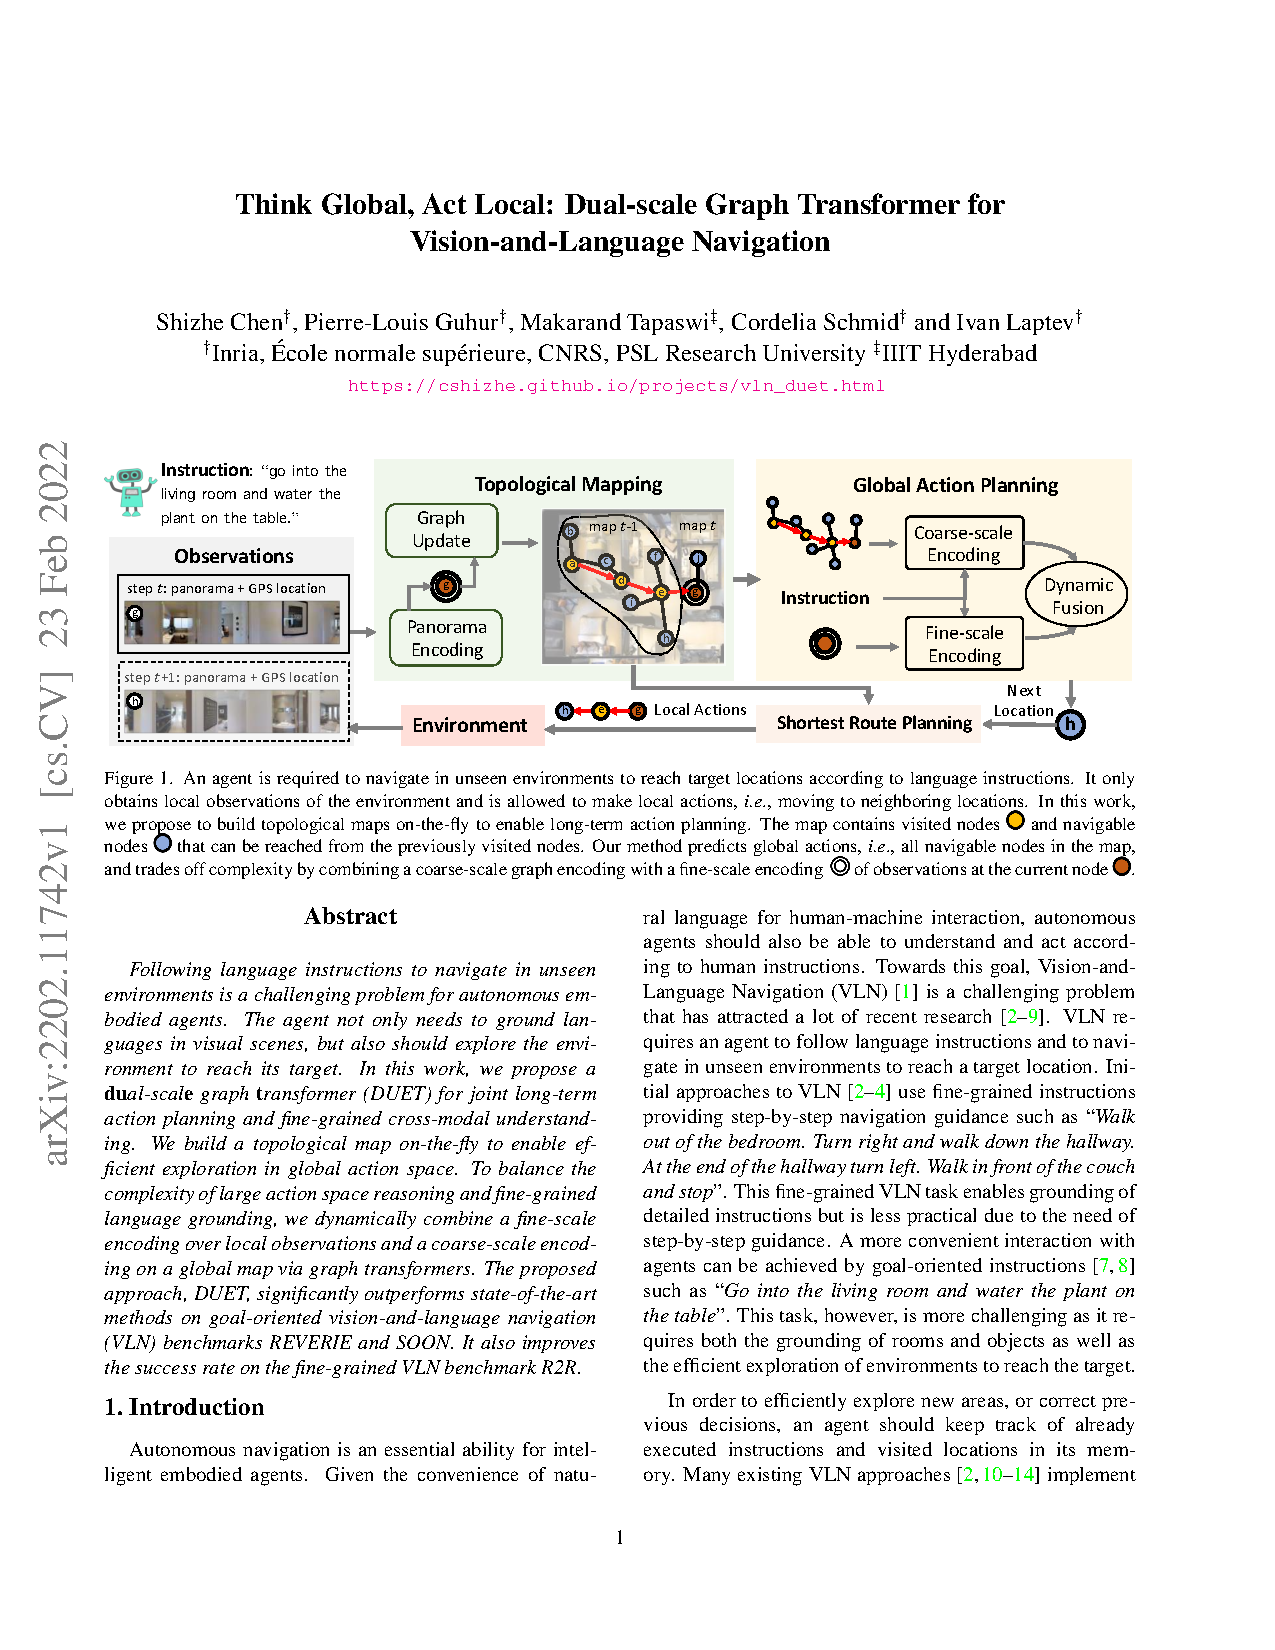
\includegraphics[page=1, width=\textwidth]{chen.pdf}
\newpage
\includegraphics[page=2, width=\textwidth]{chen.pdf}

\thesistranslationchinese
\section{全局思考,局部行动:双尺度图变换器用于视觉和语言导航}

\textbf{摘要}

在未知环境中根据语言指令进行导航对于自主体感知代理是一个具有挑战性的问题。代理不仅需要将语言与视觉场景联系起来,还需要探索环境以达到目标。在这项工作中,我们提出了一种双尺度图变换器(DUET),用于联合长期行动规划和细粒度跨模态理解。我们即时构建拓扑地图,以在全局行动空间中实现高效探索。为了平衡大规模行动空间推理的复杂性和细粒度语言基础的需求,我们通过图变换器动态结合局部观察的细尺度编码和全局地图的粗尺度编码。所提出的方法,DUET,在以目标为导向的视觉与语言导航(VLN)基准测试REVERIE和SOON上显著优于现有最先进方法。它还在细粒度VLN基准测试R2R上提高了成功率。

\textbf{引言}

自主导航是智能体化代理的基本能力。鉴于自然语言在人机交互中的便利性,自主代理也应能理解并按照人类指令行动。为实现这一目标,视觉与语言导航(VLN)是一个具有挑战性的问题,近年来吸引了大量研究关注。VLN要求代理根据语言指令在未知环境中导航以到达目标位置。最初的VLN方法使用细致的指令提供逐步导航指导,例如“从卧室走出来,向右转,沿着走廊走下去。在走廊的尽头向左转,走到沙发前停下来”。这种细致的VLN任务能够实现对详细指令的落地,但由于需要逐步指导,实际应用性较低。通过目标导向的指令可以实现与代理更便捷的交互,例如“进入客厅,给桌子上的植物浇水”。然而,这项任务更具挑战性,因为它不仅需要对房间和物体进行落地,还需要有效地探索环境以到达目标。

为了有效探索新区域或纠正之前的决策,代理需要在其记忆中记录已执行的指令和已访问的位置。许多现有的VLN方法使用循环架构(例如LSTM),并将导航历史压缩成固定大小的向量来实现记忆。可以说,这种隐式记忆机制可能无法有效存储和利用具有丰富时空结构的先前经验。一些近期方法提出明确存储之前的观察和行动,并通过变换器模型长距离依赖以预测行动。然而,这些模型只允许执行局部行动,即移动到邻近位置。因此,代理需要多次运行其导航模型以回溯步骤,这增加了不稳定性和计算量。

一种潜在的解决方案是构建一个地图 [18],该地图明确记录到目前为止观察到的所有已访问和可导航位置。地图使代理能够制定有效的长期导航计划。例如,代理可以从地图中选择一个长期目标,并使用地图计算到达目标的最短路径。拓扑地图已被之前的视觉和语言导航(VLN)工作 [8, 19, 20] 探索。然而,这些方法在两个方面仍有不足。首先,它们依赖于递归架构来跟踪导航状态,如图2中间所示,这可能极大地阻碍探索的长期推理能力。其次,拓扑地图中的每个节点通常由压缩的视觉特征表示。这种粗略的表示减少了复杂性,但可能缺乏细节,无法在指令中对细粒度对象和场景描述进行定位。

我们的方法解决了这两个缺点,第一个基于变换器架构,第二个使用双尺度行动规划方法。我们提出了一个带有拓扑地图的双尺度图变换器(DUET)。如图1所示,我们的模型由两个模块组成:拓扑映射和全局行动规划。在拓扑映射中,我们通过向地图添加新观察到的位置并更新节点的视觉表示来随时间构建拓扑地图。然后在每一步中,全局行动规划模块预测地图中的下一个位置或停止动作。为了平衡细粒度语言定位和大图推理,我们提议从双尺度动态融合行动预测:当前位置的细尺度表示和地图的粗尺度表示。特别是,我们使用变换器捕捉跨模态视觉与语言关系,并通过引入图拓扑知识来改进地图编码。我们通过行为克隆和辅助任务对模型进行预训练,并提出一个伪交互示范者来进一步提高策略学习。DUET 在面向目标的 VLN 基准测试 REVERIE 和 SOON 上显著优于最先进的方法。它还提高了细粒度 VLN 基准 R2R 的成功率。总之,我们工作的贡献有三个方面:
\begin{enumerate}
    \item 我们提出了一个用于 VLN 的双尺度图变换器(DUET),结合了粗尺度地图编码和当前位置的细尺度编码,以有效规划全局行动。
    \item 我们采用图变换器编码拓扑地图,并学习与指令的跨模态关系,以便行动预测可以依赖于长距离导航记忆。
    \item DUET 在面向目标的 VLN 基准测试上达到了最先进的水平,在挑战性的 REVERIE 和 SOON 数据集上的成功率(SR)提高了超过 20\%,同时也普遍适用于细粒度 VLN 任务,即在 R2R 数据集上将 SR 提高了 4\%。
\end{enumerate}

\end{document}
